\documentclass[dvipdfmx]{standalone}
\usepackage{tikz}
\usepackage{pgfplots}
\pgfplotsset{compat=1.18}
\begin{document}
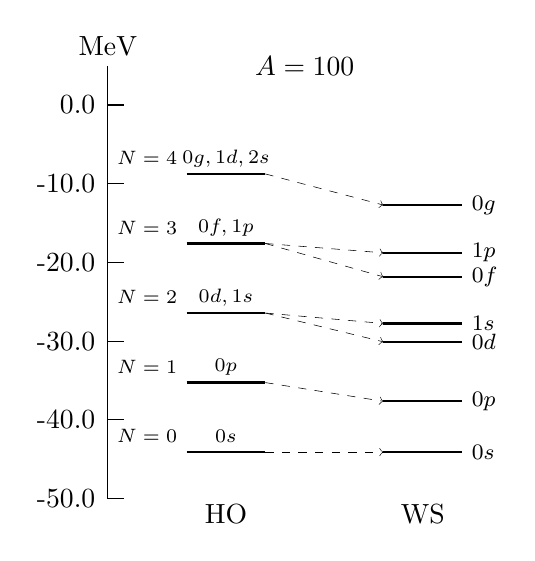
\begin{tikzpicture}

% 縦軸(エネルギーのスケール)
\draw (-0.5, -5.0) -- (-0.5, 0.5) node[above] {MeV};
\foreach \y/\text in {0.0/{0.0}, -10.0/{-10.0}, -20.0/{-20.0}, -30.0/{-30.0}, -40.0/{-40.0}, -50.0/{-50.0}} {
    \draw (-0.5, \y/10) -- (-0.3, \y/10) node[left] {\text\ \ \ };
}

% HOレベル(左側)
\node at (1, -5.2) {HO};
\foreach \n/\y/\text in {
    4/-8.757/{$0g, 1d, 2s$},
    3/-17.591/{$0f, 1p$},
    2/-26.424/{$0d, 1s$},
    1/-35.257/{$0p$},
    0/-44.09/{$0s$}} {
    \node at (0, \y/10+0.2) {\scriptsize{$N=\n$}};
    \node at (1.0, \y/10+0.2) {\scriptsize\text};
    %横線の位置(x,y)
    \draw[thick] (0.5, \y/10) -- (1.5, \y/10);
}

% WSレベル(右側)
\node at (3.5, -5.2) {WS};
\foreach \name/\y/\label in {
    0g/-12.713/58,
    1p/-18.782/40,
    0f/-21.829/34,
    1s/-27.754/20,
    0d/-30.084/18,
    0p/-37.636/8,
    0s/-44.09/2} {
    \node[anchor=west] at (4, \y/10) {\footnotesize$\name$};
    \draw[thick] (3, \y/10) -- (4, \y/10);
}

% 矢印(HOからWSへの接続)
\if0
\foreach \y in {0.0, -10.0, -20.0, -30.0, -40.0, -50.0, -60.0} {
    \draw[->] (0.5, \y/10) -- (4, \y/10);
}
\fi

\draw[very thin,dashed,->] (1.5,-44.09/10) -- (3,-44.09/10);
\draw[very thin,dashed,->] (1.5,-35.257/10) -- (3,-37.636/10);
\draw[very thin,dashed,->] (1.5,-26.424/10) -- (3,-30.084/10);
\draw[very thin,dashed,->] (1.5,-26.424/10) -- (3,-27.754/10);

\draw[very thin,dashed,->] (1.5,-17.591/10) -- (3,-21.829/10);
\draw[very thin,dashed,->] (1.5,-17.591/10) -- (3,-18.782/10);
\draw[very thin,dashed,->] (1.5,-8.757/10) -- (3,-12.713/10);

\node at (2.0,0.5) {$A=100$};
\end{tikzpicture}
\end{document}
